\chapter{実装}\label{chap:implementation}

本章では、人間と計算への指示を融合させたプログラミング環境の具体的な実装について述べる。
全体の概要について述べた後、個別の要素について詳しく説明する。

\section{Babascriptプログラミング環境}\label{babascriptux30d7ux30edux30b0ux30e9ux30dfux30f3ux30b0ux74b0ux5883}

本研究では、第\ref{chap:design}章にて設計した人間と計算への指示を融合させたプログラミング環境の
具体的な実装として、Babscriptプログラミング環境を提案する。
Babascriptプログラミング環境では、人間をコンピュータと同じ計算資源として扱うことで
実世界におけるタスクの処理など、人間の力を最大限活用した新しい処理を実現可能である。
以下の要素を組み合わせることによって実現する。

\begin{itemize}
\itemsep1pt\parskip0pt\parsep0pt
\item
  Babascript
\item
  Babascript Agent
\item
  Node-Linda
\end{itemize}

Babascriptは人間への指示を記述可能にするプログラミングライブラリである。
Babascript Agentは、指示に対する実行結果を入力できるソフトウェアだ。
Node-Lindaは、Babascript及びBabascript
Agentの間のデータ通信の仲介サーバとして機能する。

以下のような手順で、処理が進む。

\begin{enumerate}
\def\labelenumi{\arabic{enumi}.}
\itemsep1pt\parskip0pt\parsep0pt
\item
  人への指示構文を実行する (Babascript)
\item
  指示内容がNode-Lindaサーバを経由してクライアントへと配信される
  (Node-Linda)
\item
  指示を受け取ったクライアントがユーザに処理を促す (Babascript Agent)
\item
  指示実行者が、指示に従って行動し、その結果を入力する (Babascript
  Agent)
\item
  Node-Lindaサーバを経由して実行元プログラムに入力された処理結果が送信される
  (Node-Linda)
\item
  プログラム側で指定されたコールバック関数が実行される (Babascript
  Agent)
\end{enumerate}

Babascriptプログラミング環境の概要を図\ref{fig:system_image}に示す。

\begin{figure}[htbp]
  \begin{center}
  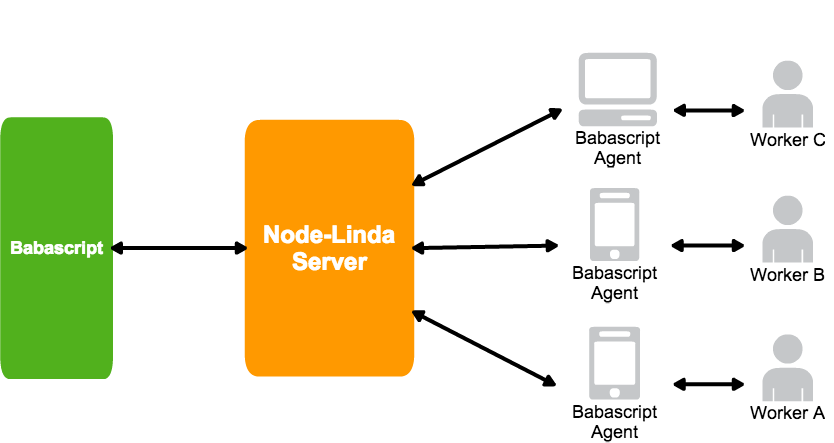
\includegraphics[width=.7\linewidth,bb=0 0 834 443]{images/overview.png}
  \end{center}
  \caption{システム概要}
  \label{fig:system_image}
\end{figure}

以下の節において、個別の要素に関して詳しく述べる。

\section{Babascript}\label{babascript}

プログラムと人とのインタラクションを実現するためには、プログラム上で人間への指示を行える仕組みが必要だ。
そこで、Babascriptという、人間への指示構文を持ったオブジェクト(以下、人間オブジェクト)を宣言できるプログラミングライブラリを実装した。
BabascriptはJavascriptのサーバサイド実行環境であるNode.js及びRuby上で動作する。
本論文で示すサンプルソースコードは全てJavascriptで記述したものを掲載する。

\subsection{基本仕様}\label{ux57faux672cux4ed5ux69d8}

Babascriptでは、人間オブジェクトを通して人間とプログラムのメッセージングを行う。
通常のメソッド実行とほぼ同じ記法で人間への指示を送ることができる。
つまり、オブジェクトにメッセージングするという従来のオブジェクト指向プログラミングの作法をそのまま実行することで
人間に指示を送っている。
例えば、ソースコード:\ref{code:babascript-sample}のようなプログラムによって、人間オブジェクトを宣言し、人間へ指示を送ることができる。

\begin{lstlisting}[caption=人への指示構文, label=code:babascript-sample]
// ライブラリの読み込み
var Babascript = require('babascript');
// takumibabaという人間を対象とした人間オブジェクトの宣言
var takumibaba = new Babascript('takumibaba');
// takumibabaに対して"clean_up_your_room"という指示を送る
takumibaba.clean_up_your_room();
\end{lstlisting}

人間オブジェクトは生成時にidを指定する必要がある。
人への指示構文は、このidを元に命令配信先を決定する。 例えば、id=baba
に命令を送りたい場合、人オブジェクト宣言時の第一引数にはbabaという文字列を指定する。
指定したidに命令が配信されるため、Babascript
Agent側でも同じidを指定する必要がある。

人間オブジェクトは、自身に定義されていないメソッドが実行されると、エラーを返さずに、人間への指示として解釈する。
そのため、実装されていないメソッド名であれば、あらゆる命令をメソッドとして表現し実行することが可能である。
例えば、「toString」や「call」等のメソッドは、javascriptにおいてはほぼすべてのオブジェクトが持つメソッドだ。
一方で、「clean\_up\_your\_room」や「bake\_bread」のようなメソッドは定義しない限りは存在しないメソッドである。
Babascriptは、この定義されていないメソッドをエラーとして評価せず、
人への指示構文として評価する(ソースコード:\ref{code:methodmissing-sample})。

\begin{lstlisting}[caption=通常のメソッドと指示構文の例, label=code:methodmissing-sample]
var Babascript = require('babascript');
var baba = new Babascript('takumibaba');

baba.exists_method = function(){return true}

// 上記で定義したメソッド, 人への命令構文ではない
baba.exists_method();
// 既に定義されているメソッド, 人への命令構文ではない
baba.toString();

// 定義されていないメソッド, 人への命令構文として解釈される
baba.not_exists_method();
\end{lstlisting}

オブジェクトに存在しないメソッドが呼び出された時に、特定のメソッドにその処理を委譲するような仕組みは、
プログラミング言語Rubyにおいてはmethodmissingと呼ばれる。
各言語によって名称は異なるが、類似する仕組みが存在する言語は複数存在する。
Babascriptにおいては、node-methodmissing\footnote{https://github.com/geta6/node-methodmissing}というライブラリを利用している。

また、ソースコード
\ref{code:babascript-exec-method}のように、execメソッドを使うことで指示を送ることも可能だ。
execメソッドを利用する場合は、第一引数に命令内容、第二引数にオプション情報、第三引数にコールバック関数を指定する。

\begin{lstlisting}[caption=execメソッドによる指示構文, label=code:babascript-exec-method]
var Babascript = require('babascript');
var takumibaba = new Babascript('takumibaba');

takumibaba.exec("message_to_human", {}, function(result){
  // 処理を記述する
});
\end{lstlisting}

人間への指示として評価されたメソッドは、そのメソッド名と引数を元にしたタスク情報を生成し、タスク配信サーバへと送信する。
この際、メソッド名部分がユーザに命令として提示される文となる。
タスク情報はソースコード\ref{code:task-format}のように構成される。

\begin{lstlisting}[caption=タスク情報の例, label=code:task-format]
var task = {
  name: "takumibaba", // 命令配信先ID
  key: "instruction_body", // 指示内容
  cid: "1420569060.52_0.9777606867719442", // タスクID
  type: "eval", // 命令のタイプ
  option: { // オプション情報
    format: "boolean", // 想定返り値型
  }
}
\end{lstlisting}

メソッド名が自由に設定できるため、内容は指示ではなく、質問のようなものもあり得るが、本研究では統一して指示と呼ぶ。
人への指示構文の第一引数にはオプション情報を指定する。
第二引数には人力処理の実行後に実行するコールバック関数を指定する。
このコールバック関数は、指示に対して何かしらの値が返されたときに実行される。

\subsection{オプション情報の付加}\label{ux30aaux30d7ux30b7ux30e7ux30f3ux60c5ux5831ux306eux4ed8ux52a0}

メソッド名以外に送信したい情報があるときには、第一引数にオプション情報としてオブジェクトを与える。
クライアントアプリケーション側でオプション情報を得ることができるため、このオプション情報に応じて
ユーザに提示する画面を変更するといったことが可能である。

オプション情報の例としては、返り値の型情報や、タイムアウト情報などが考えられる。
オプション情報はソースコード\ref{code:babascript-option}のように記述する。
この場合であれば、返り値の型はstringで、3分後までに返り値を得られなかった場合は、
人力処理を止め、第二引数で指定するコールバック関数を実行し、処理を続行させるといったことをオプション情報として記述している。

\begin{lstlisting}[caption=オプション情報のサンプルソースコードその1, label=code:babascript-option]
var Babascript = require('babascript');
var baba = new Babascript('takumibaba');

baba.hogefuga({format: 'string', timeout: 1000*60*3}, function(){

});
\end{lstlisting}

また、ソースコード:\ref{code:babascript-option-list}の場合であれば、listで指定した選択肢の中から選んで返り値を返す、といった指定が可能だ。

\begin{lstlisting}[caption=オプション情報のサンプルソースコードその2, label=code:babascript-option-list]
var Babascript = require('babascript');
var takumibaba = new Babascript('takumibaba');

var option = {
  format: 'string'
  list: ['良い', '普通', '悪い']
};
takumibaba.会場の雰囲気はどうですか(option, function(result){
  // 人が処理した結果が引数に格納される。
  // 返り値に応じて処理を分岐させる
  if(result.value == '良い'){
    // ...
  }else if(result.value == '普通'){
    // ...
  }else if(result.value == '悪い'){
    // ...
  }else{
    // ...
  }
});

\end{lstlisting}

特別なオプション情報として、broadcastとinterruptが存在する。
broadcastオプションは、同じ指示を複数のワーカーに同時に配信し、指定した数だけの値を得ることが出来た場合に
コールバック関数を実行するというものだ。
指定した数の値が集まらない場合でも、コールバック関数を実行させることもできる。
タイムアウトオプション等と組み合わせ、5分経ったら得られた値のみを使って処理を継続する、といったことが可能だ。
interruptオプションは、他の指示が先に送られていた場合でも、指示が溜まったキューに割り込んで指示を追加することのできる
オプションである。
現在実行されているタスクの次のタスクとして登録される。

オプション情報である第一引数は省略可能である。
省略した場合は、自動的にソースコード:\ref{code:option-default}のようなオブジェクトが代入される。

\begin{lstlisting}[caption=デフォルトのオプション情報, label=code:option-default]
var defaultOption = {
  format: 'boolean'
}
\end{lstlisting}

\subsection{コールバック関数の指定}\label{ux30b3ux30fcux30ebux30d0ux30c3ux30afux95a2ux6570ux306eux6307ux5b9a}

人への指示構文の第二引数に関数を代入すると、実行結果を取得した後に指定した関数を実行する。
処理が成功していた場合、この関数に渡される第二引数の中に、実行結果が代入される。
処理が失敗していた場合、第一引数にエラーの内容が代入される。
人間は計算機の処理に比べて遅延しがちであるため、非同期を前提とした実装をしている(ソースコード:\ref{code:babascript-callback})。

\begin{lstlisting}[caption=コールバック関数の指定, label=code:babascript-callback]
var Babascript = require('babascript');

var baba = new Babascript('takumibaba');
baba.do_callback({format: 'boolean'}, function(result){

});
\end{lstlisting}

また、Promiseによる処理関数の指定も可能である。
人への指示構文実行時、コールバック関数を指定しなかった場合、Promiseオブジェクトがその時点での返り値として返される。
Promiseオブジェクトのthenメソッドに指示に対する処理結果が得られた場合に実行する関数を、
catchメソッドに何かしらのエラーが起きて結果を得られなかった場合に実行する関数を指定する(ソースコード:\ref{code:babascript-promise})。

\begin{lstlisting}[caption=Promiseによる関数指定, label=code:babascript-promise]
var takumibaba = new Babascript("takumibaba");

takumibaba.use_promise({}).then(function(result){
  // 実行結果が正しく得られた場合の処理を記述する
}).catch(function(error){
  // エラー等で実行結果が得られなかった場合の処理を記述する
});
\end{lstlisting}

\subsection{コマンドラインでの利用}\label{ux30b3ux30deux30f3ux30c9ux30e9ux30a4ux30f3ux3067ux306eux5229ux7528}

Babascriptはコマンドラインツールとしても利用可能だ。
babaコマンドは、ソースコード:\ref{code:baba-command}のように利用することができる。
オプションeの直後に指示内容を、オプションnの直後に指示先のIDを指定する。
format情報などを付加したい場合は、オプションoの後に key=value
の形で指定することができる。
コマンドラインで実行することによって、人間による処理をpipeに組み込むといったことも可能になる。

\begin{lstlisting}[caption=Babaコマンド, label=code:baba-command]
% baba -e hogefuga -o format=boolean
\end{lstlisting}

\section{Babascript Agent}\label{babascript-agent}

Babascriptによって人への指示をプログラムに記述し、実行することが可能となったが、その指示を人に伝え、
処理結果を返させるためのアプリケーションが必要となる。
そこで、Babascript Agent というアプリケーションを実装した。 Babascript
Agent
は、Babascriptとの通信を担うサービス部と返り値の入力等を担うインタフェース部から構成される。

\subsection{サービス}\label{ux30b5ux30fcux30d3ux30b9}

サービス部は、主にBabascriptとのやりとり、つまり、命令の受け取りや返り値の送信などを担う。

命令を受け取ると、イベントを発行する

\begin{lstlisting}[caption=Babascript Agent サービス部のソースコード例, label=code:babascript-client-service]
var Client = require('babascript-client');

var client = new Client("takumibaba");
client.on("get_task", function(task){
  // babascriptからの命令を受信した時の挙動を記述
});

client.on("cancel_task", function(task){
  // 命令が何かしらの理由でキャンセルされた時の挙動を記述
});
\end{lstlisting}

何かしらの値を実行結果として返すときは、clientオブジェクトに実装されているretrnValueメソッドを用いる。
ソースコード:\ref{code:babascript-client-service-returnvalue}のように、第一引数に結果として返すものを指定する。

\begin{lstlisting}[caption=Babascript Agent 処理結果を返すメソッドの例, label=code:babascript-client-service-returnvalue]
var Client = require('babascript-client')l
var client = new Client('takumibaba');

client.returnValue(true);
client.returnValue(10);
client.returnValue("string");
\end{lstlisting}

実行結果情報として返すデータの例を図\ref{code:return-value-data}に示す。

\begin{lstlisting}[caption=タスク情報, label=code:return-value-data]
value = {
  _task: task, // 元タスクのオブジェクト情報
  value: true, // ワーカーが入力する実行結果
  cid: '1420569060.52_0.9777606867719442', // タスクのID情報
  worker: 'takumibaba', //実行者情報
  options: {},
  type: "return"

}
\end{lstlisting}

命令実行をキャンセルしたい場合は、cancelメソッドを用いる。
cancelメソッドの第一引数に、キャンセルする理由を指定することができる。

\subsection{ユーザインタフェース}\label{ux30e6ux30fcux30b6ux30a4ux30f3ux30bfux30d5ux30a7ux30fcux30b9}

ユーザとのインタラクションを行う。
命令をユーザに見せるのと、実際に実行結果を入力させる機能を持つ

サービス部と独立した実装のため、異なるデバイスや環境上でもインタフェース部を実装するだけでBabascript
Agentの機能を構築可能である。
指示内容と返り値の入力インタフェースをユーザに提示し、返り値の入力を受け付ける機能を担う。
この際、Babascriptの指示でオプション情報として返り値の型を指定していた場合、指定した型以外の入力を受け付けないような実装を行っている。
返り値の型は現在、Boolean, String, Numberに対応している。

例として、スマートフォンアプリケーション、slackインタフェースを実装した。

\subsubsection{スマートフォンアプリケーション
プロトタイプ1}\label{ux30b9ux30deux30fcux30c8ux30d5ux30a9ux30f3ux30a2ux30d7ux30eaux30b1ux30fcux30b7ux30e7ux30f3-ux30d7ux30edux30c8ux30bfux30a4ux30d71}

インタフェースの例として、スマートフォンアプリケーションとして実装した。
HTMLとJS、CSSによるwebアプリケーションとして実装し、 Apache
Cordova\footnote{http://cordova.apache.org/}を用いてスマートフォンアプリケーション化した。
android及びiOSアプリケーションとして動作する。
JavascriptのフレームワークにはBackbone.js\footnote{http://backbonejs.org/}とMarionette.js\footnote{http://marionettejs.com/}を利用している。
CSSはSASS\footnote{http://sass-lang.com/}、HTMLはJade\footnote{http://jade-lang.com/}で記述した。
システムは図\ref{fig:client-overview}のように構成される。

\begin{figure}[htbp]
  \begin{center}
  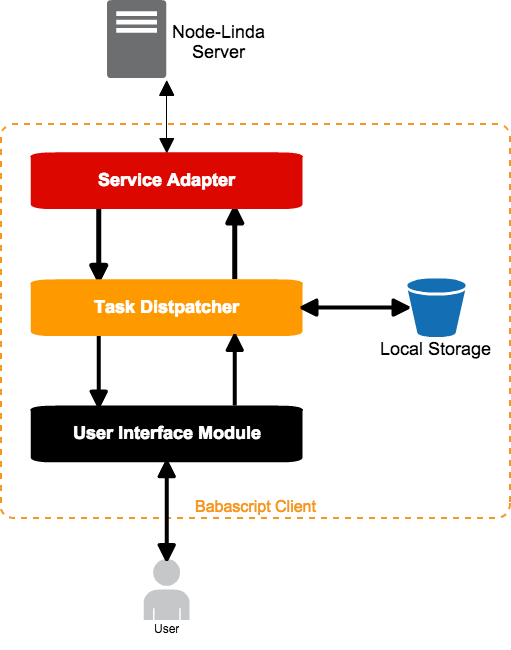
\includegraphics[width=.5\linewidth,bb=0 0 511 650]{images/client-overview.png}
  \end{center}
  \caption{Babascript Agent webアプリケーションシステム図}
  \label{fig:client-overview}
\end{figure}

Webインタフェースでは、指示内容に応じて提示インタフェースを変化させる実装をしている。
例えば、フォーマットにBooleanを指定していた場合、ユーザには「はい」と「いいえ」の2種類のボタンが提示される。
それぞれのボタンにはtrueとfalseの値が設定されており、ボタンを押すことによって設定された値を返り値としてプログラムに送ることができる。
また、StringとNumberであれば、文字・数字の入力フォームと投稿ボタンが提示され、
投稿ボタンを押した際にフォームに入力されていた内容が返り値としてプログラムに返される。
Listであれば、選択フォームが表示され、リストの中から返り値を選択することができる。
実際に提示されるインタフェースの例を図\ref{fig:client_format_list}に示す。

\begin{figure}[htbp]
  \begin{center}
  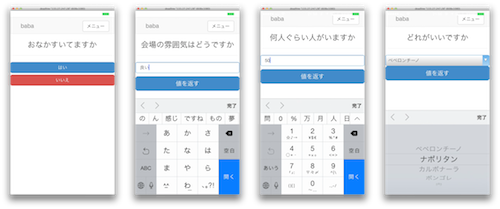
\includegraphics[width=.8\linewidth,bb=0 0 500 209]{images/client_format_list.png}
  \end{center}
  \caption{Babascript Agent Webアプリケーションインタフェース}
  \label{fig:client_format_list}
\end{figure}

プログラムからの指示を受け取ると、アプリによる通知を発行し、ユーザに値を返すよう促す(図\ref{fig:client-push-notification})。

\begin{figure}[htbp]
  \begin{center}
  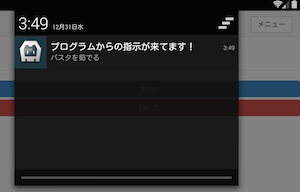
\includegraphics[width=.5\linewidth,bb=0 0 300 192]{images/client-push-notification.png}
  \end{center}
  \caption{Babascript Agent Push通知例}
  \label{fig:client-push-notification}
\end{figure}

指示が実行できない場合には、エラーを値として返すことができる。
例えば、自宅にいるにも関わらず、大学の研究室にいないと出来ないような指示が来た場合には、少なくともその時点では
指示を実行に移すことは出来ない。
エラー処理のインタフェースを図\ref{fig:throw-error}に示す。

\begin{figure}[htbp]
  \begin{center}
  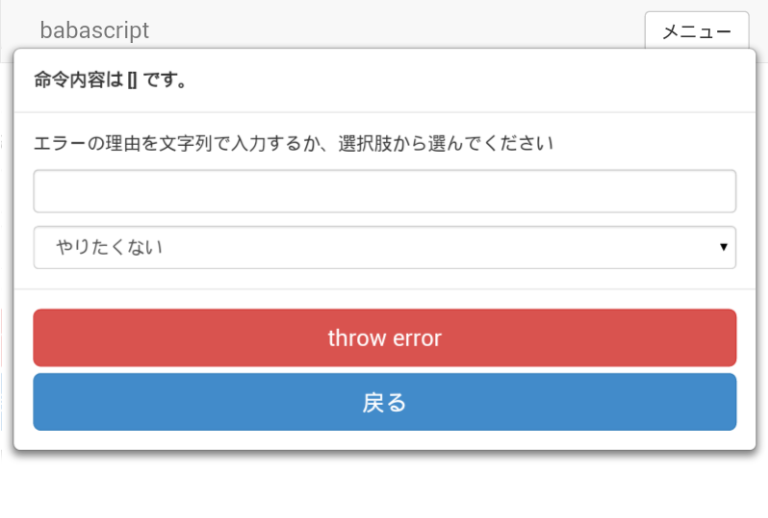
\includegraphics[width=.5\linewidth,bb=0 0 768 518]{images/throw-error.png}
  \end{center}
  \caption{Babascript Agent エラー処理インタフェース}
  \label{fig:throw-error}
\end{figure}

\subsubsection{スマートフォンアプリケーション
プロトタイプ2}\label{ux30b9ux30deux30fcux30c8ux30d5ux30a9ux30f3ux30a2ux30d7ux30eaux30b1ux30fcux30b7ux30e7ux30f3-ux30d7ux30edux30c8ux30bfux30a4ux30d72}

プロトタイプ1では、複数の指示が受けた場合でも一つ一つの指示しか表示できなかった。
人間は実世界で様々な処理を並列で実行していることから、Babascript
Agentにおいても 取得した指示を並列に示すことが望ましい。

そこで、基本的なインタフェースはプロトタイプ1を踏襲し、受けた指示の一覧をTODOリスト風のインタフェースを用いて
ワーカーに提示するアプリケーションを実装した。
こちらのアプリケーションをプロトタイプ2とする。

\subsubsection{チャットボット}\label{ux30c1ux30e3ux30c3ux30c8ux30dcux30c3ux30c8}

チャットサービス上で稼働するボットにBabascript Agentの機能を実装した。
ボットシステムにはHubot\footnote{https://hubot.github.com/}を採用した。
Hubotは様々なチャットサービスに対応しているが、Slackというチャットサービス上において運用している。
このボットシステムは、Heroku\footnote{https://heroku.com}上で稼働している。
チャットボットのシステム図を図\ref{fig:babascript_client_hubot_system}に示す。

\begin{figure}[htbp]
  \begin{center}
  \includegraphics[width=.3\linewidth,bb=0 0 273 402]{images/babascript_client_hubot_system.png}
  \end{center}
  \caption{Hubotシステム図}
  \label{fig:babascript_client_hubot_system}
\end{figure}

チャットボットシステムは、ユーザからのメッセージによる問い合わせに応じて返答を行う。
返答の例を図\ref{fig:babascript_client_slack}に示す。

\begin{figure}[htbp]
  \begin{center}
  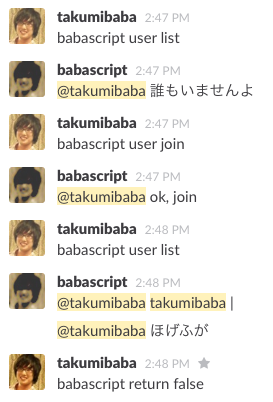
\includegraphics[width=.4\linewidth,bb=0 0 273 402]{images/babascript_client_slack.png}
  \end{center}
  \caption{Babascript Agent Slackインタフェース}
  \label{fig:babascript_client_slack}
\end{figure}

チャットボットインタフェースでは、Webアプリケーションの場合と違い、
提示するインタフェースを返り値の型に応じて変化させるといったことができない。
そのため、ユーザにとっては値を返しにくくなっているが、普段利用しているチャットサービス上で
Babascript Agentの機能を利用できるということは有用なことであると考える。

\section{通信手法}\label{ux901aux4fe1ux624bux6cd5}

BabascriptとBabascript
Agent間の通信のために、仲介サーバとしてNode-Linda\cite{node-linda}を利用する。
通信手法はデバイスごとに利用可能な手法が異なったり限定されるため、プラガブルにする必要がある。
そこで、接続方式の追加などを容易に実装可能なNode-Lindaを仲介サーバとして採用した。

Babascript及びBabascript
AgentがNode-Lindaに接続するために実装されたモジュールを、Babascript
Adapterと呼ぶ。
このAdapterは切り替えが可能で、かつ他の実装に影響を与えることがないように設計されている。
Babascript及びBabascript
AgentはこのAdapterを介してNode-Lindaに接続し、情報のやりとりを行う。

本節では、この仲介サーバとして用いるNode-Lindaについて述べた後、2種類のBabascript
Adapterを紹介する。

\subsection{Node-Linda}\label{node-linda}

\subsubsection{概要}\label{ux6982ux8981}

Node-Linda\cite{node-linda}は、分散並列処理のための仕組みであるLinda\cite{linda}をNode.js上に実装したものだ。
Lindaは、タプルスペースという共有メモリを用いてプロセス間でデータの通信を行う並列処理のためのモデルだ。
Node-Lindaでは、Lindaを拡張し、ネットワーク経由でも利用できるようにしている。
ネットワーク経由での利用のため、あらゆるプログラミング言語から利用可能だ。
接続のためのプログラムさえ記述すれば、あらゆるデバイスがNode-Lindaに接続可能である。
Linda及びNode-Lindaのタプル空間への操作を表\ref{table:tuple-management}にまとめる。

\begin{longtable}[c]{@{}lcc@{}}
\caption{Linda及びNode-Lindaのタプル空間への操作
\label{table:tuple-management}}\tabularnewline
\toprule
操作 & Linda & Node-Linda\tabularnewline
\midrule
\endfirsthead
\toprule
操作 & Linda & Node-Linda\tabularnewline
\midrule
\endhead
書き込み & out & write\tabularnewline
読み込み & rd & read\tabularnewline
読み込みつつ削除 & in & take\tabularnewline
ブロックして読み込み & rdp & -\tabularnewline
ブロックして読み込みつつ削除 & inp & -\tabularnewline
書き込みを読み続ける & - & watch\tabularnewline
\bottomrule
\end{longtable}

watch操作は従来のLindaの仕様にはなく、Node-Linda独自の仕様である。
また、Node-Lindaでは非同期処理が前提となっており、ブロック処理は仕様から削除されている。

実世界コンピューティングでの利用を前提としており、様々なセンサーやアクチュエータが接続することが想定される。
Babascriptによる人間の指示実行結果も、センサーやアクチュエータの処理を同じようにNode-Linda上で共有される。
つまり、Node-Linda上において人間はセンサーやアクチュエータと同じような存在になる。

Node-Lindaの各操作は、ソースコード\ref{fig:linda-usage}のようなプログラムで実現する。

\begin{lstlisting}[caption=Node-Lindaへの接続方法, label=code:linda-usage]
// Node-Lindaに接続するクライアントの準備
var LindaClient = require('linda').Client;
var socket = require('socket.io-client').connect('http://babascript-linda.herokuapp.com/');
var linda = new LindaClient().connect(socket);

// タプルスペース(共有メモリ空間)の宣言
var tuplespace = linda.tuplespace('babascript');

// タプルスペースへの書き込み
tuplespace.write({"type": "sensor"});

// タプルスペースからデータを読み込む
tuplespace.read({}, function(err, data){
  //
});

// タプルスペースからデータを読み込んで消す
tuplespace.take({}, function(err, data){

});

// タプルスペースへのデータ書き込みを監視する
tuplespace.watch({}, function(err, data){

});

tuplespace.cancel(cid);
\end{lstlisting}

\subsubsection{Node-Lindaのタプル操作}\label{node-lindaux306eux30bfux30d7ux30ebux64cdux4f5c}

Babascript及びBabascript
Agentは、Adapterを用いてNode-Lindaのタプルスペースの操作を行う。
宣言時に指定するIDを元に使用するタプルスペースを決定する。
通常の指示を書き込むnormalスペース、割り込み処理用に使うinterruptスペースを個別に利用することで、
割り込み処理を優先的に読み込ませるようにしている。

\subsection{Socket.IO Adapter}\label{socket.io-adapter}

Socket.IO
Adapterは、リアルタイム通信のためのライブラリであるSocket.IO\footnote{http://socket.io/}を用いて
Node-Lindaに接続するためのAdapterだ。
WebsocketもしくはXHR-Pollingによって常にNode-Lindaサーバと通信をし続ける。
全ての処理はSocket.IOによる通信によって実現する。

常時通信している都合上、バッテリー消費の問題が生じたり、デバイスによっては通信を強制的に切断されてしまうことがある。
Socket.IO Adapterは、接続環境が良好な状態での利用が望ましい。
例えば、常設型のコンピュータ等においての利用が想定される。

構成図を図\ref{fig:socket.io-adapter}に示す。

\subsection{PushNotification Adapter}\label{pushnotification-adapter}

PushNotification Adapter は、HTTP
RequestとPushNotificationを用いてNode-Lindaと通信を行うためのAdapterだ。
Cordovaのプラグインとして実装した。 Node-Lindaへのタプル操作はHTTP
Requestの実行によって実現する。
Node-Linda側からAdapter側への通信には、PushNotificationを用いる。 Amazon
AWS
SimpleNotificationService\footnote{http://aws.amazon.com/jp/sns/}を利用し、
PushNotificationを実現している。 PushNotification
Adapterを利用するためには、Node-Linda側でPushNotification
Adapter用のライブラリを読み込む必要がある。

PushNotification
Adapterは、モバイルデバイス等の常時接続が難しいデバイス上で、可能な限りリアルタイムなやりとりを実現するために
実装された通信モジュールだ。
主にAndroidやiPhone等のモバイルデバイスからNode-Lindaと接続する際に利用する。

構成図を図\ref{fig:push-notification-adapter}に示す。

\begin{figure}[htbp]
  \begin{center}
  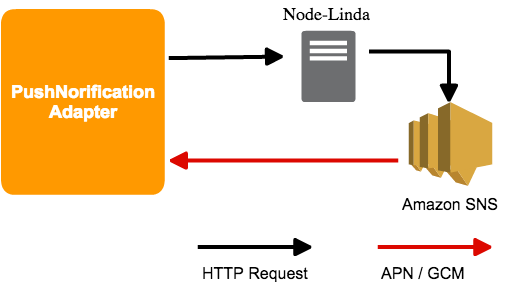
\includegraphics[width=.5\linewidth,bb=0 0 529 303]{images/push-notification-adapter.png}
  \end{center}
  \caption{PushNotification Adapter}
  \label{fig:push-notification-adapter}
\end{figure}

\section{プラグイン機構}\label{ux30d7ux30e9ux30b0ux30a4ux30f3ux6a5fux69cb}

Babascript 及びBabascriptClient
Agentはその機能を拡張するために、プラグイン機構を持つ。

図\ref{code:babascript-plugin}の様に使うことで、Babascript及びBabascript
Agentによってイベントが発生した時に、
それに応じたデータを受け取り、自由に操作することができる。

\begin{lstlisting}[caption=Babascript Plugin, label=code:babascript-plugin]
var Babascript = require('babascript');
var baba = new Babascript('takumibaba');

var Client = require('babascript-client');
var client = new Client('takumibaba');

var logger = require('babascript-plugin-logger');

baba.set logger()
\end{lstlisting}

Babascript及びBabascript Agent
は、表\ref{table:plugin-events}にあるイベントを受け取る。
また、イベントを受け取った際にはイベントに応じたデータを受け取る。

\begin{longtable}[c]{@{}lrr@{}}
\caption{Babascript及びBabascript Agentが発行するイベント一覧
\label{table:plugin-events}}\tabularnewline
\toprule
イベント名 & Babascript & Babascript Agent\tabularnewline
\midrule
\endfirsthead
\toprule
イベント名 & Babascript & Babascript Agent\tabularnewline
\midrule
\endhead
load & ○ & ○\tabularnewline
connect & ○ & ○\tabularnewline
send & ○ & ×\tabularnewline
return\_Value & × & ○\tabularnewline
receive & ○ & ○\tabularnewline
\bottomrule
\end{longtable}

loadイベントは、プラグインが読み込まれた際に発生する。
例えば、設定ファイルの読み込みなどの処理を行う。

connectイベントは、Babascript及びBabascript
AgentがNode-Lindaサーバに接続した際に発生するイベントだ。
sendイベントは、Babascriptによって人間への指示構文が実行された際に発生する。
例えば、指示内容を全てログとして保存したいときなどには、sendイベントと共に受け取るデータを送信するといったことができる。

return\_valueイベントは、Babascript
Agentが指示に対して実行結果を返すときに発生する。
receiveイベントは、Babascript及びBabascript
Agentが何かしらのデータをNode-Lindaサーバから受け取る際に発生する。
指示を送ってから値が帰ってくるまでの時間を計測したいときなどは、このイベントをフックするプラグインを実装する必要がある。

プラグイン機構によって、Babascript環境を拡張していくことが容易となる。

\section{まとめ}\label{ux307eux3068ux3081}

人間と計算機の処理を融合させたプログラミング環境の具体的な実装や利用方法について述べた。
